% author: Tomas Trnka
% mail: tomas@trnkatomas.eu
% date: 2013-07-04

\documentclass[a4paper,10pt]{article}
%\usepackage[czech]{babel}
%\usepackage[T1]{fontenc}
\usepackage[hmargin=2.2cm,vmargin=2.2cm]{geometry}
\usepackage[utf8x]{inputenc}
\usepackage{fancyhdr}
\usepackage{amsmath} 
\usepackage{tikz}
\usetikzlibrary{patterns}
\usetikzlibrary{calc}
\usepackage{enumerate}
\pagestyle{fancy}
\headheight 15pt
\lhead{Crpyto, Fall 2014}
\rhead{Tomas Trnka}
\def\firstcircle{(270:1.75cm) circle (2.5cm)}
\def\secondcircle{(150:1.75cm) circle (2.5cm)}
\def\thirdcircle{(30:1.75cm) circle (2.5cm)}
\begin{document}
\section*{DES}
\begin{enumerate}[a)]
\item Let's consider one Feistel round which is the essential part of the DES cipher.

\begin{figure}[h!]
\centering
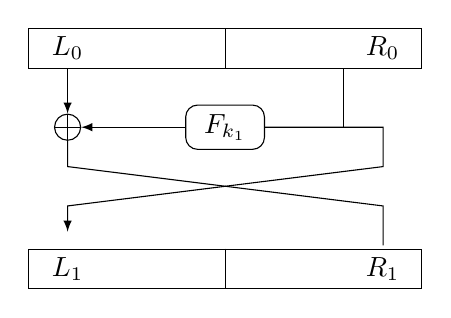
\begin{tikzpicture}
\foreach \z in {1} {
\node (f\z) at ($\z*(0,-1.5cm)$) [minimum width=1cm,rounded corners=1ex,draw] {$F_{k_\z}$};
\node (xor\z) [left of = f\z, circle, node distance = 2cm, draw] {};
\draw[-] (xor\z.north) -- (xor\z.south);
\draw[-] (xor\z.east) -- (xor\z.west);
\draw[-latex] (f\z.west) -- (xor\z.east);
}
\foreach \z in {1} {
\draw[-latex] (f\z.east) -| +(1.5cm,-0.5cm) -- ($(xor\z) - (0,1cm)$) -- ($(xor\z.north) - (0,1.5cm)$);
\draw[-] (xor\z.south) -- ($(xor\z)+(0,-0.5cm)$) -- ($(f\z.east) + (1.5cm,-1cm)$) -- +(0,-0.5cm);
}
\node (p0) [above of = f1, minimum width=5cm,minimum height=0.5cm,node distance=1cm,draw] {}; 
\node (l0) [above of = xor1,node distance=1cm] {$L_0$};
\node (r0) [right of = l0, node distance = 4cm] {$R_0$};
\draw[-] (p0.north) -- (p0.south);
\draw[-latex] (l0 |- p0.south) -- (xor1.north);
\draw[-] ($(f1.east)+(1.0cm,0)$) -- +(0,0.75cm);
\node (p1) [below of = f1, minimum width=5cm,minimum height=0.5cm,node distance=1.8cm,draw] {}; 
\draw[-] (p1.north) -- (p1.south);
\node (l1) [below of = xor1,node distance=1.8cm] {$L_1$};
\node (r1) [right of = l1, node distance = 4cm] {$R_1$};
\end{tikzpicture}  
\end{figure}

In our case we have the inputs for the Feistel round $c(L_0)$ and $c(R_0)$.
We have to examine the $F$ function to realize what is going on inside it:
\begin{figure}[h!]
\centering
\begin{tikzpicture}
\node (p0) [above of = f1, minimum width=5cm,minimum height=0.5cm,node distance=1cm,draw] {}; 
\node (l0) [above of = p0,node distance=0cm] {$32 b$};
\node (E) [below of = p0, minimum width=1cm,minimum height=1cm,node distance=1.2cm,draw] {E}; 
\draw[-latex] (p0) -- (E.north);
\node (p1) [below of = E, minimum width=6cm,minimum height=0.5cm,node distance=1.5cm,draw] {}; 
\node (l1) [above of = p1,node distance=0cm] {$48 b$};
\draw[-latex] (E.south) -- (p1);
\node (xor) [below of = p1, circle, node distance = 1cm, draw] {};
\draw[-] (xor.north) -- (xor.south);
\draw[-] (xor.east) -- (xor.west);
\draw[-latex] (p1) -- (xor.north);
\node (key) [right of = xor, minimum width=4cm,minimum height=0.5cm,node distance=6cm,draw] {48b key}; 
\draw[-latex] (key) -- (xor.east);
\node (p2) [below of = xor, minimum width=6cm,minimum height=0.5cm,node distance=1.2cm,draw] {}; 
\node (p_a) [left of = p2, minimum width=0cm,minimum height=0.5cm,node distance=2.8cm] {}; 
\node (l2) [above of = p2,node distance=0cm] {$48 b$};
\draw[-latex] (xor.south) -- (p2.north);
\node (s1) [below of = p_a, minimum width=0.8cm,minimum height=0.5cm,node distance=1.2cm,draw] {$S_1$};
\foreach \z [evaluate = \zz using int(\z-1)] in {2,3,...,8} {
\node (s\z) [right of = s\zz, minimum width=0.8cm,minimum height=0.5cm,node distance=0.8cm,draw] {$S_\z$}; 
}
\node (end) [below of = p2, minimum width=5cm,minimum height=0.5cm,node distance=2.6cm,draw] {32b}; 
\foreach \z in {1,2,...,8} {
\draw[-latex] (p2.south) -- (s\z.north);
\draw[-latex] (s\z.south) -- (end.north);
}
\end{tikzpicture}  
\end{figure}

\begin{enumerate}
\item On the input we have got 32b $c(R_0)$, the expansion function works only with the bits of original input and just build bigger block, do not flip the bits and therefore we can claim that $c(E(R_0)) = E(c(R_0))$. 
\item Now we have to know what the key scheduler does with the key. The scheduler just creates permutations of the original key, so it also does not flip any of the bits of the original key. So we can also be sure that our $K_1'$ is equal to the $c(K_1)$
\item no we have to perform the $XOR$ calculation with these two inputs.
\begin{eqnarray*}
E(c(R_0)) \oplus K_1' &=& c(E(R_0)) \oplus c(K_1)\\
c(E(R_0)) \oplus c(K_1) &=& (E(R_0)\oplus 1^{48}) \oplus (K_1 \oplus 1^{48}) \\
\end{eqnarray*}
Since the the $\oplus$ is commutative and holds that $1^{48he result of} \oplus 1^{48} = 0^{48}$ we can rewrite the equation as:
$$
E(R_0) \oplus K_1
$$
which is exactly the same as we would obtain with the not bitwise flipped inputs. So the rest of the function $F$ continues through the $S$ blocks and outputs the same value as it would for the normal inputs.

The last step of Feistel round is to $XOR$ the output of $F_k$ with $c(L_0)$. Since we know that $F(K_1',c(R_0)) = F(K_1,R_0)$ we can write:
\begin{eqnarray*}
c(L_0) \oplus F(K_1,R_0) &=& 1^{32}\oplus L_0 \oplus F(K_1,R_0)\\
1^{32}\oplus L_0 \oplus F(K_1,R_0) &=& 1^{32} \oplus R_1\\
\end{eqnarray*}
and the result is exactly $R_1$ bitwise flipped. This property is preserved for all the 16 rounds of DES and therefore we can say that it is true that $c(y) = DES(c(K),c(M))$.
\end{enumerate}
\item We can say that because of this property the search space for the exhaustive method will be 2 times smaller. The reason is because when we send plain text attack message $M$, we obtain some output $DES_k(M)$ and as we show in the previous bullet we can simply obtain the result for $DES_{c(k)}(c(M))$ just by flipping bitwise the previous result considering this operation quick enough.

So encoding only one message we can obtain two results, instead of trying both keys $k_i$ and $c(k_i)$ just one will be enough. Therefore we have to try only half of the keys, which means that instead of $2^{56}$ we have to try $\frac{2^{56}}{2}=2^{55}$ possibilities for the key.

\end{enumerate}
\end{document}